\chapter{Results}
\label{chap:res}
In this section we will present and discuss the results from the experiments on the REST implementation. The experiments were conducted on an Intel(R) Xeon(R) Gold 6426Y processor with 500 GB RAM. Samples from the Porto dataset are used as data.

To describe different variants of REST, labels for each variant have been created. The spatial filter variant is denoted by the suffix \textit{-SFX}, where \textit{X} is the window size in meters. The Sakoe-Chiba band is denoted by the suffix \textit{-BNDX}, where \textit{X} is the band size. The KNN variant is denoted by the suffix \textit{-KNNX}, where \textit{X} is the number of MRTs selected. An example label can be \textit{REST-SF75-KNN3-BND20}, this represents REST using a spatial filter with window size $75\times75 m^2$, selecting the 3 best MRTs, and applying a Sakoe-Chiba band of size 20 to each Max DTW calculation.

\section{Compression Ratio and Runtime}
These experiments have been executed by first building a reference set with a sample size of 10K, to then use the reference set for compression. The trajectories in the sample used to build the reference set were excluded from the later compression, since they would have a much higher compression ratio than other trajectories.

\begin{figure}[h]
    \begin{minipage}{0.99\linewidth}
        \centering
        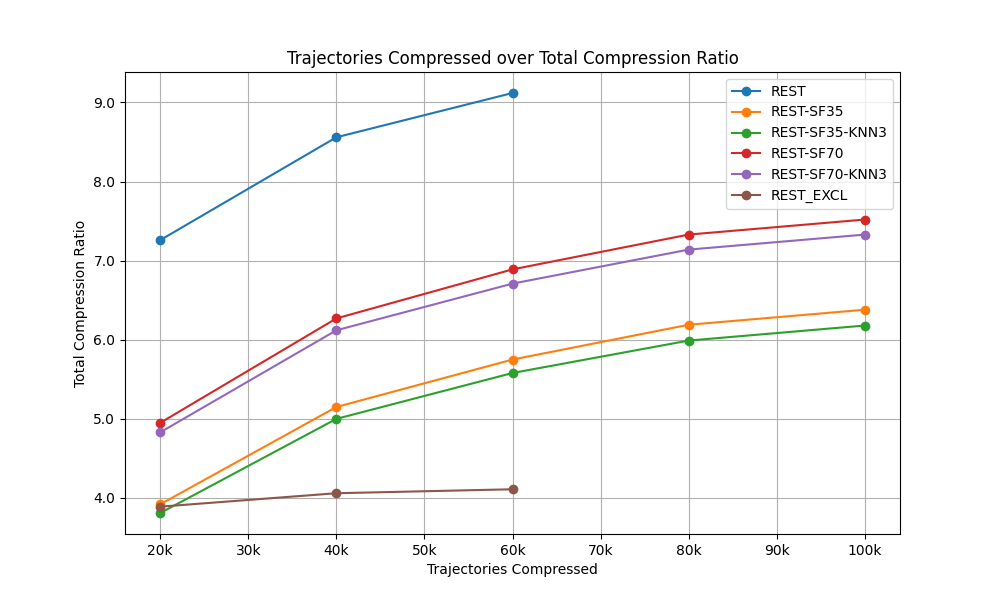
\includegraphics[height=7cm, keepaspectratio]{../code/plotting/tot_compression.png}
        \caption{Total Compression Ratio over trajectories compressed. The reference set was constructed using a sample size of 10K.}
        \label{fig:n_compression}
    \end{minipage}
\end{figure}

In figure \ref{fig:n_compression} it is clear that REST has the best compression ratio. It has a total compression ratio of 9.12 for 60K compressed trajectories, which is high. The spatial filter variants have a lower compression ratio, but it increases with a larger window size. This is expected because REST can be seen as having an infinitely large window size. The KNN variants in combination with spatial filter shows promising results as they only slightly reduce the compression ratio compared to spatial filter with no KNN. KNN used directly on REST did not show promising results and is not shown in the results. This is likely because REST uses all reference trajectories to search for MRTs, selecting a handful early in the process seems to miss out on better suggestions.

In general the total compression grows as more trajectories are compressed. This is because the number of compressed trajectories grows larger in relation to the set size. From equation \ref{eq:tot_cr}, this represents \textit{points\_in\_set} becoming smaller compared to \textit{all\_points}. In the case where the amount of compressed trajectories keeps growing, the size of the reference set would eventually become negligible, causing the total compression to approach the average compression. The average compression ratio (not shown), stays near the same level for all variants, around 14.5 for REST. Moreover, the amount of compressions needed to make the reference set negligible is much larger than any realistic use case. The result in our experiments is that the total compression grows slower and slower.

XREST has a much slower growth than the other variants, this is because XREST has a smaller reference set. Thereby, noticing less of a change as the number of trajectories compressed increase. It also has a much lower compression ratio than REST. This indicates in combination with the exclusive strategy of XREST indicates that the reference set has low coverage. XREST needs a larger sample size in order to gain coverage, experiments covering this, are discussed in section \ref{sec:sample_size}.

\begin{figure}[h]
    \begin{minipage}{0.99\linewidth}
        \centering
        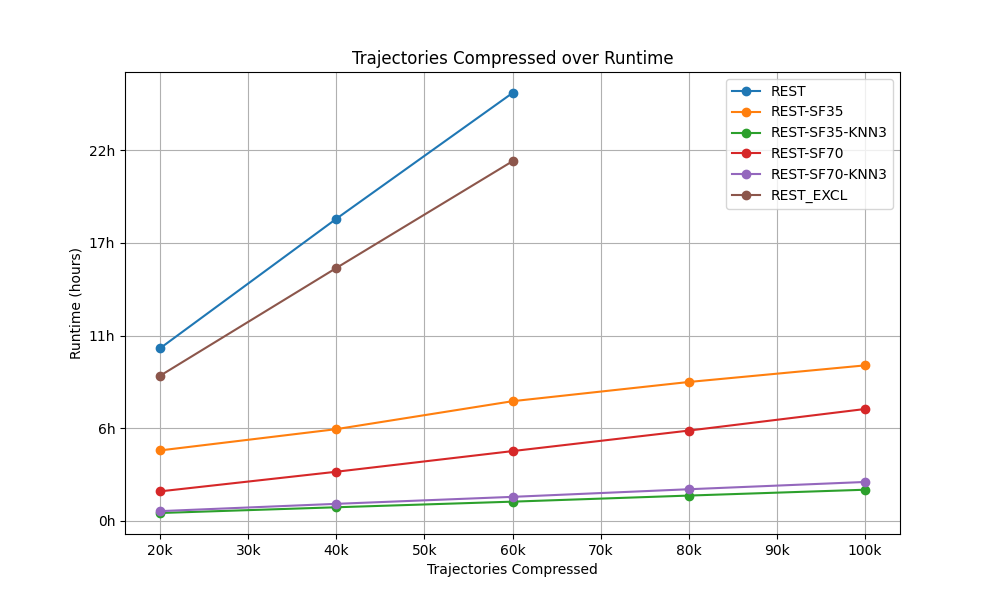
\includegraphics[height=7cm, keepaspectratio]{../code/plotting/n_runtime.png}
        \caption{Runtime over trajectories compressed. The reference set construction is included in the time, using a 10K sample size.}
        \label{fig:n_runtime}
    \end{minipage}
\end{figure}

In figure \ref{fig:n_runtime} we see that REST and XREST are significantly slower than other variants. This demonstrates the inefficiency of using the entire reference set as candidates in MRT search. XREST is slightly faster than REST, this is because the reference set is smaller, leading to less reference trajectories to search through. Although, with a smaller reference set we would expect XREST to be even faster. This indicates that the quality of the reference set is slowing it. XREST has shorter trajectories in the reference set, causing a more segmented compression sequence.

The spatial filter variants are significantly faster than REST and XREST. The spatial filter efficiently selects a subset of the reference set to use for MRT search. Note that \textit{REST-SF70} is faster than \textit{REST-SF35}, this is unexpected as a smaller window size is expected to find candidate reference trajectories, and hence do fewer trajectory comparisons. Nonetheless, the smaller window size is slower, this is because the reference set is bigger. When using a smaller window size, fewer trajectories are found in reference set construction as well, leading to a larger set. With the larger set, there are more trajectories even within the smaller window size, leading to a slower runtime.

We see that the KNN variants in combination with a spatial filter leads to a faster runtime. Interestingly, the gap between \textit{REST-SF70} and \textit{REST-SF35} is larger than the gap between the corresponding variants with KNN. This means that when using KNN, a larger window size has less impact on the runtime than without KNN.

All in all, looking at both compression ratio and runtime, we see that the spatial filter variants are much faster than REST and XREST, while reaching high compression ratios. REST itself is slow, but achieves high compression ratio by using the entire reference set for each compression. XREST has the lowest compression ratio and the second-highest runtime. This indicates the strategy is unable to compete with REST using this sample size.

None of the variants have a compression ratio as good as REST, but we see a trend that increasing window size also increases compression ratio. The increased window size also leads to a higher runtime. However, using KNN in addition to spatial filter seems to mitigate this somewhat. This demonstrates that a spatial filter in combination with KNN is a good middle way, achieving high compression ratio with a low runtime.

\section{Sample Size testing}\label{sec:sample_size}
These experiments were executed by compressing 100K trajectories using higher sample sizes. This resulted in reference sets with increasing coverage. The effect sample size has on the total compression ratio and the average compression ratio will be discussed in this section. Due to time constrains, results for REST and XREST could not be generated, as increasing the sample size also increases the runtime significantly. However, we believe the sped-up variants will show the same patterns as the REST and XREST.

\begin{figure}[h]
    \begin{minipage}{0.99\linewidth}
        \centering
        \includegraphics[height=7cm, keepaspectratio]{../code/plotting/sample_size_tot.png}
        \caption{Total compression over Sample Size from compressing 100K trajectories.}
        \label{fig:sample_tot}
    \end{minipage}
\end{figure}

In figure \ref{fig:sample_tot}, \textit{REST-SF35-KNN3} has the highest compression ratio for a sample size of 20K, the compression ratio gradually declines as the sample size grows beyond this. As the sample size grows, so does the set size. In order achieve a better compression ratio with a larger set, the compression gain must be large. The slow decline indicates that there is some compression gain, which is outweighed by the increase in set size. The optimal balance between compression and set size is struck using a sample size of 20K, reaching a total compression ratio of $6.44$.

\begin{figure}[h]
    \begin{minipage}{0.99\linewidth}
        \centering
        \includegraphics[height=7cm, keepaspectratio]{../code/plotting/sample_size_avg.png}
        \caption{Average compression over Sample Size from compressing 100K trajectories. Average compression is the average compression ratio of each compressed trajectory, without taking the reference set size into account.}
        \label{fig:sample_avg}
    \end{minipage}
\end{figure}

In figure \ref{fig:sample_avg}, the average compression ratio is shown. The difference between total and average compression is the inclusion or exclusion of the reference set size. The average compression is interesting because it gives insight into the coverage of the reference set. Without taking the reference set size into account this ratio simply shows how well each trajectory is compressed on average. As the sample size increases the average compression ratio also increases. This is expected, because more reference trajectories gives a higher coverage reference set.

However, the growth of the average compression is decreasing, even as the sample size increases. If there is no gain in average compression when sample size increases, this must mean that the coverage of the reference set is approaching 100\%. Because no new information is gained from using a larger sample in reference set construction.

The results in figure \ref{fig:sample_avg} are based on compressing 100K trajectories of a total 1.7M in the dataset. Because the compressed trajectories are randomly selected from the dataset, it is very unlikely that the characteristics of the selected subset is significantly different from the rest of the set. Therefore, it is safe to assume that the resulting average compression for N = 100K, would be similar for N = 1M. Since the characteristics of the dataset would be similar for the additional trajectories compressed. Assuming the average compression ratio stays the for a higher N, this would lead to a better total compression.

All in all, the results from varying sample sizes show that a reference set with high coverage can be built using a small sample size relative to the dataset. The average compression grows as coverage increases, while the total compression reaches an optimal point and then declines as the reference set grows in size.